\chapter{Implementación}

\section{Frameworks}

\subsection{No funcionales}

Para la implementación de nuestro sistema, originalmente, evaluamos la
utilización de distintos frameworks disponibles. DeepQA, el producto
de IBM, no es de código abierto, por lo que acerca de su
implementación sólo sabemos lo que ventilaron en sus artículos
técnicos. Just.ask, el sistema basado en web comparado contra
OpenEphyra no está disponible en la web al momento de escribir este
trabajo, mientras que OpenEphyra no funciona tal cual está dise\~nado
originalmente (basado en web), sino que el autor sugiere unos pasos
esotéricos para configurarlo para usar conocimiento local. Cabe
destacar que esta falla en la funcionalidad está asociada a la que
había encontrado [AUTOR DE PAPER EPHYRA1] en Aranea y está
vinculado con una serie de medidas restrictivas tomadas por las
compa\~nías de buscadores, que fueron cerrando sus accesos gratuitos
para la comunidad de investigación bloqueando sus APIs y el acceso
automático a sus UI. Las alternativas para el uso de buscadores,
actualmente, se reducen a la configuración de una serie de proxies
sobre los que rotar el acceso a la UI y así enga\~nar al detector de
accesos automáticos -alternativa de legalidad cuestionable - o bien al 
pago por una quota de queries por mes.
OpenEphyra sobrevivió a Aranea porque sus responsables escribieron
una interfaz para Bing cuando Google cerró sus puertas, mientras que
los responsables de Aranea no lo hicieron. Finalmente, Bing también
bloqueo el acceso automático gratuito. Notar que el mismo tipo de
discontinuación ocurrió con el API de traducciones de Google. La
empresa declara, explícitamente, que no está dispuesta a acceder a
ninguna quota de acceso gratuito para la investigación académica y
que todos sus servicios son pagos. 

%Tanto de Aranea como de OpenEphyra podríamos llegar a tomar algunos de
%sus componentes a la hora de construir nuestro sistema. Por el momento,
%fueron simplemente dejados de lado.

\bigskip

\subsection{Qanus}

Finalmente, un sistema que \textit{sí} estaba disponible y funcionando
fue Qanus, que respetaba al pie de la letra su detalle técnico. Al comienzo
del proyecto, contábamos con un corpus de datos en XML,
lo cual coincidía, al menos en gran parte, con el input esperado de
la implementación Qa-sys. A pesar de esto, la adaptación de los
componentes no fue nada trivial y requirió un tiempo excesivo. En
particular, existían dos opciones a la hora de construir un sistema
sobre la arquitectura Qanus: dejar de lado la implementación Qa-sys e
implementar todos los componentes de cero sobre la arquitectura, respetando las interfaces
dadas por el framework, o adaptar el sistema funcionando para que
trabaje sobre los nuevos datos y el nuevo entorno esperado. Frente a
esta alternativa, se aparece claro que el framework en sí mismo no
aporta demasiado, pues lo único que hace es atar la implementación
final a una interfaz estructurada de tres procesos bastante sencillo.
Además, existe un cierto grado de dependencia de la arquitectura
hacia la implementación final, quizás no a nivel técnico, pero si
en el modo en el que está definida la estructura. Por este motivo,
encaramos una adaptación de Qa-sys a nuestro modelo de datos y a
nuestros requerimientos, pero los resultados no fueron buenos en
términos de resultados por tiempo invertido. El tiempo de aprendizaje
del framework mismo y el tiempo requerido para adaptar las distintas
componentes propias a las interfaces esperadas por Qanus es demasiado
alto para la solución que brinda. Como recién mencionamos, en
realidad, el proceso de pipeline de tres pasos no tiene tantas aristas,
y adaptarse a un framework es mucho menos ameno que escribirlo. Este
puede ser uno de los motivos por los cuales, como acertadamente
se\~nalan los autores de Qanus, no existe ningún framework
estandarizado dentro del ámbito de la investigación en QA.
Después de la investigación inicial, podríamos concluir que
está estandarizado, al menos a modo conceptual, la idea de que la
resolución del problema se debe enfocar como un pipeline de al menos
tres pasos que incluyen:
\begin{itemize}
\item el preprocesamiento de la base de conocimiento,
\item el preprocesamiento de la pregunta,
\item el retorno de la respuesta a partir de los resultados de los dos pasos anteriores. 
\end{itemize}
Como último comentario al respecto, el modelo de Qanus resultaba poco atractivo
 a la hora de incorporar procesamiento en varios idiomas: el mejor approach
utilizando esta arquitectura era implementar dos sistemas basados en
Qanus paralelos y utilizar uno u otro de acuerdo con el resultado de
una detección inicial. 

\bigskip

Si bien el modelo de Qanus fue, por los motivos recién expuestos,
dejado de lado, debemos destacar una serie de puntos en los que fue
útil.

En primer lugar, uno de los objetivos de Qanus es facilitar el ingreso
al área del QA de nuevos investigadores. Creemos que esto está
logrado perfectamente: el código es muy sencillo y claro y lo mismo
ocurre con la documentación, lo que hace de Qanus un proyecto muy
útil desde una perspectiva pedagógica o educativa, más allá de
que sea esta misma simpleza la que más adelante atente contra la
usabilidad. El modelo de pipeline, que es el enfoque teórico usual al
problema, y los distintos componentes y usos típicos de estos
componentes en los distintos pasos del pipeline se realizan linealmente
en la implementación de Qanus y Qa-sys. En particular, la similaridad
entre la descripción del código de IBM (DeepQA y Watson) y el
enfoque con el que Qanus ataca el mismo problema salta a la vista,
considerando la diferencia de escalas. 

En segundo lugar, en el plano de la investigación del estado de arte
de los sistemas de QA disponibles creemos que el intento con Qanus
redundó en un cierto escepticismo sobre la posibilidad de resolver
nuestro problema utilizando herramientas disponibles de gran escala. La
conclusión es análoga a la que tuvo el equipo de IBM al intentar
usar OpenEphyra y PIQUANT: el tiempo de customización y adaptación
de los framework a nuestro problema puntual es demasiado alto en
comparación con el tiempo necesario para construir una nueva
arquitectura que cumpla los mismos requisitos. 

Por último, en un nivel técnico, Qanus nos resultó de utilidad para
construir nuestro modelo final pues reutilizamos varios de los
componentes de Qa-sys: En primer lugar, recuperamos el POS tagger, el
NER tagger y el Question Classiffier (QC) de Stanford, que son las
librerías principales con las que Qa-sys encara el procesamiento
lingüístico de la pregunta y parte del proceso de generación de
respuestas. Todas estas herramientas están disponibles en la web por
otros medios, pero algunas -principalmente el QC- requieren un cierto
tiempo de configuración inicial que los autores de Qanus ya habían
resuelto. Es decir, reutilizamos, además de estos módulos externos,
bastante de la configuración y las APIs de acceso a estos módulos
escritos por los singapurenses. Estas herramientas funcionan bien
sólo para inputs en inglés. Las adaptaciones que hicimos las
veremos más abajo. Por otro lado, incorporamos casi sin
modificaciones algunas métricas de distancia entre pasajes que Qa-sys
usa en el momento de la generación de la respuesta como Scorers.
Estos son las clases: \textbf{FeatureSearchTermCoverage},
\textbf{FeatureSearchTermFrequency}, \textbf{FeatureSearchTermProximity},
\textbf{FeatureSearchTermSpan}. Explicaremos esta métricas en breve, dentro de nuestro
modelo, bajo en nombre de
{\textquotedblleft}Comparadores{\textquotedblright}. Este código
está escrito por los autores de Qanus (es decir, no es una librería externa utilizada por ellos).


\bigskip

\section{Arquitectura}

\subsection{Motivación}

Después del intento con Qanus, decidimos implementar el sistema por
fuera de cualquier framework y encaramos el dise\~no actual. En este
dise\~no respetamos el modelo típico de pipeline de tres pasos que
abunda en la literatura científica y, por lo demás, parece el
indicado a la hora de encarar este tipo de problemas. Un momento no-técnico
importante a destacar es la obtención de una base de datos en
mongodb, resultado del trabajo del proyecto MITIC, la cual cambió
sustancialmente el enfoque anterior, basado en XMLs. 
A partir de estos datos, fue posible delinear un esquema de entidades formal que determinó
qué se puede responder y qué no. Como vimos, la estrategia de QA
cuando el tipo de datos es estructurado es radicamente distinta que la
estrategia cuando los datos son no estructurados. Qanus, por su parte,
está orientado a un tipo de datos no estructurados: buscar documentos
rankeados en un índice de búsqueda y rastrear en ellos pasajes
mediante distintos métodos. Cuando la base de conocimientos consta de
un tipo de datos estructurado (esto es, de entidades, relaciones,
atributos de entidades) es posible delimitar una ontología más
rígida que permita concentrarse en la interpretación de la pregunta
hacia un lenguaje formal. El arquetipo de este enfoque puede pensarse
como la traducción de un lenguaje de consulta humano a un lenguaje de
consulta formal, como por ejemplo, SQL: esta estrategia de QA puede
entenderse \ como una interfaz inteligente a una base de datos. \ En
eje principal en este acercamiento está en el análisis
lingüístico de la pregunta a fin de mapearla a un dominio conocido
y, por otro lado, no es necesario hacer análisis lingüístico
sobre el corpus de datos.

Por otro lado, dado que nuestro objetivo inicial incluía desarrollar
métodos de QA con soporte bilingüe basados en textos (datos no estructurados) 
y esta base de conocimiento no lo permite, incorporamos al proyecto la resolución
algunos de los ejercicios de la competencia QA4MRE (Question Answering for Machine Reading Evaluation)
de la CLEF (Cross-Language Evaluation Forum) del a\~no 2007. 

Estos ejercicios fueron elegidos para poder evaluar nuestros métodos de análisis lingüsticos,
ya que la naturaleza del dominio de conocimiento del proyecto mitic - por el formato de sus datos
 y por lo puntual de su temática- hace imposible cualquier métrica de evaluación objetiva.
Tras investigar distintas competencias y métodos de evaluación, optamos por la CLEF del 2007
por contar con un subconjunto de ejercicios bastante adecuados para nuestro sistema mientras que el corpus
de datos necesario para completar estos ejercicios estaba (en parte) disponible dentro de los tiempos 
requeridos por nuestro proyecto. 

\bigskip

\subsection{Modelo}

Nuestro sistema resuelve dos problemas de QA similares pero distintos. 

Por un lado, disponemos de una base de datos estructurada, con datos del área de la investigación y la
producción en TICs en Argentina, que requiere un enfoque estructurado con métodos basados en ontologías y en 
formalizaciones de dominio. El enfoque aquí es traducir la pregunta formulada en lenguaje humano a un lenguaje más
formal ``comprensible" según el modelo de dominio. 

Por otro lado, para evaluar métodos de QA 
para datos no estructurados, resolvimos algunos ejercicios de la competencia CLEF del '07. La base de conocimientos para
estos ejercicios son algunos snapshots de Wikipedia en Espa\~nol y en Inglés, anteriores al 2007. Sobre esta base de conocimiento,
el enfoque no es ``traducir" la pregunta a un lenguaje estructurado sino interpretarla y ``compararla", mediante distintas métricas, 
con documentos y pasajes, buscando medidas estádisticas y otras condiciones que permitan \textit{rankear} una respuesta candidata
con un cierto grado de confianza, o bien determinar que no fue posible encontrar una respuesta para la pregunta. 


Conceptualmente, el modelo consiste en los tres pasos típicos: la
creación de la base de conocimientos optimizada, el análisis
lingüístico de la pregunta y la generación de una respuesta desde
la base de conocimientos optimizada a partir de la pregunta con sus
anotaciones. 
Los pasos 1 y 2, la generación de la base de conocimientos optimizada y el procesamiento de la pregunta son procesos
esencialmente análogos para la base de conocimientos estructurada y para la no estructurada. El tercer paso, la generación de respuestas,
tiene distintos enfoques según el caso. 
En las siguientes secciones recorreremos ambos enfoques en conjunto, señalando las decisiones de dise\~no y los distintos módulos
utilizados, haciendo las distinciones pertinentes cuando sea necesario.

En las secciones subsiguiente comentaremos las implementaciones de los
distintos pasos, con sus decisiones de dise\~no y las tecnologías
utilizadas. 


\bigskip

\section{Base de conocimiento}
\bigskip


La creación de la base de conocimiento es el único que se ejecuta offline
y consiste en la obtención del corpus original y en la generación de índices
invertidos. Los índices invertidos, recordamos, son índices que permiten
buscar, para una serie de términos vinculados lógicamente, un conjunto
ponderado de documentos pertinentes. Por su naturaleza, este paso está 
separado de la ejecución del resto del código.

\subsection{Corpus inicial}

\subsubsection{Grafo Mitic}
Los datos originales del proyecto mitic constan de una serie de documentos 
xml y de cinco colecciones de mongodb y relaciones entre ellas (una base de datos no relacional).

Las cinco coleccciones son: universidades, investigadores, empresas,
publicaciones, proyectos y temáticas.

Estas colecciones definen el dominio. Cada entidad 
posee sus respectivos atributos y distintas relaciones con otras entidades.
Estas relaciones contienen desde vínculos explicitos como "trabajar-en"
pero también relaciones inferidas mediante distintos algoritmos durante el proyecto mitic.
Las relaciones que incorporamos tienen distintos pesos según este tipo de caracteristicas
y tejen un grafo de distancias más o menos "especulativas" entre todas las entidades.

Los atributos de cada entidad se pueden ver en el Anexo: [[HACER Y LINKEAR]].

\subsubsection{Wikipedia}
El subset de ejercicios de CLEF'07 que elegimos resolver
utiliza como corpus un snapshot de wikipedia en inglés y otro en español,
ambos anteriores al año 2007.
El set de preguntas completo involucra una serie de documentos para los cuales hay que 
registrarse en la asociación: algunas preguntas se responden en base a wikipedia y otras en base a estos documentos.
Identificamos las preguntas que se responden desde wikpedia chequeando los documentos fuente de las respuestas esperadas.

Wikipedia ofrece diferentes formas para obtener una propia imagen de la enciclopedia.
Es posible incorporar la base de datos de wikipedia a una instalación wikimedia
propia, es posible descargar una imagen estática del sitio en archivos html y también se puede
descargar un archivo xml gigante con todos los artículos. 

En la guía para los participantes de la competencia \cite{Clef07} hay un link para descargar 
wikipedia en inglés preprocesada de Noviembre de 2006 \footnote{\url{http://ilps.science.uva.nl/WikiXML/}} y dos opciones para descargar wikipedia en español: una imagen estática en html de Noviembre de 2006 \footnote{\url{http://static.wikipedia.org/downloads/November_2006/es/}} y un dump xml de Diciembre de 2006 
\footnote{\url{http://download.wikimedia.org/images/archive/eswiki/20061202/pages-articles.xml.bz2}}

La guía aclara que, bajo responsabilidad de los participantes, se puede usar
cualquier otra versión de Wikipedia, siempre y cuando sea anterior a noviembre / diciembre de 2006.
Además, se pide que las respuestas sean tomadas de ``entradas reales" o artículos de wikipedia y
no de otros documentos (por ejemplo: ``image", ``discussion", ``category", etc).

Los links a páginas de wikipedia en español no estaban más disponibles (ambos respondieron 404), mientras que el formato
preprocesado pedido para el inglés resultaba realmente complejo de instalar y parecía una linea muerta. Por estos motivos,
seguimos la sugerencia sobre el uso responsable de otras wikipedias y utilizamos las siguientes:

\medskip

\begin{center}
\begin{tabular}{ | l | l | l |}
    \hline
    Idioma & Fecha & Tamaño\\ \hline
    Inglés \footnote{\url{http://dump-ingles-1}} & 4 de noviembre de 2006 & 7,6G \\ \hline
    Español \footnote{\url{http://dump-español-1}} & 7 de julio de 2006 & 558M \\ \hline
\end{tabular}  
\end{center}

El mantenimiento de un mismo formato para ambos idiomas nos permitió crear un indexador único para cualquier
dump en xml de una wikipedia. Durante el desarrollo y las pruebas, para evitar tiempos de carga innecesarios y también
para probar, utilizamos otras imagenes disponibles de wikipedia:

\medskip

\begin{center}
\begin{tabular}{ | l | l | l |}
    \hline
    Idioma & Fecha & Tamaño\\ \hline
    Español & 26 de enero de 2007 & 902M \\ \hline
    Español & 14 de junio de 2013 & 7,3G \\ \hline
    Inglés simple & 4 de julio de 2006 & 26M \\ \hline
    Inglés simple & 24 de julio de 2013 & 406M \\ \hline
 \end{tabular}
\end{center}


\subsection{Creación de Indices}

\begin{figure}[H]
  \centering
    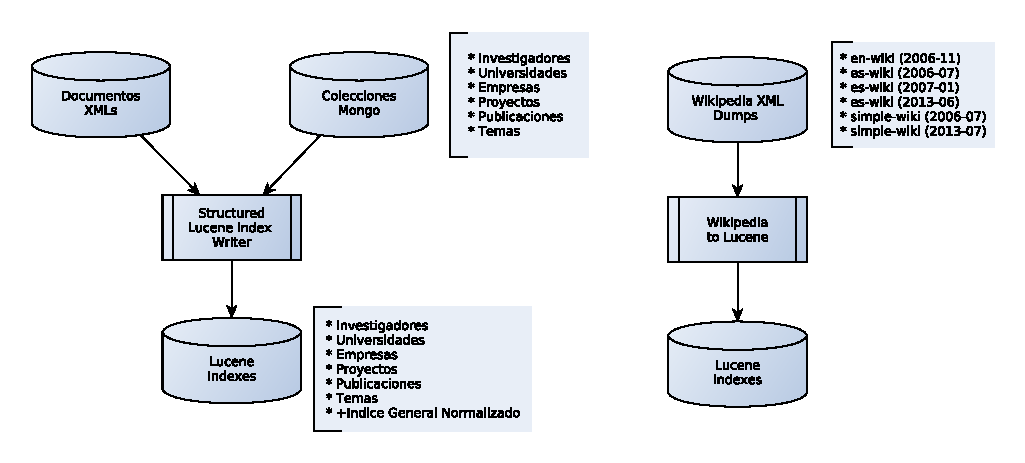
\includegraphics[scale=0.86]{graficos/LuceneWritersJuntos}
  \caption{Creación de Indices}
  \label{fig:LuceneIndexWriterBoth}
\end{figure}

A partir de esta base de datos de mongo y de los archivos xml fueron construidos cinco índices
de búsqueda lucene y un índice de búsqueda más, general, con la
información normalizada de los otros cinco. 
Cada uno de los cinco índices por entidad mantiene la estructura del tipo como campos de los documentos.
Esto quiere decir que el índice invertido para \emph{Investigadores} tiene los mismos campos
del modelo de datos de nosql. Además, se agregó el campo ``all" que resulta de la concatenación de
todos los campos. Este campo resulta útil a la hora de filtrar resultados. 
El índice general posee un documento por cada entidad de las cinco colecciones, 
manteniendo también un puntero a la entidad original y su tipo.
%El proceso de creación de índices se ilustra en la Figura \ref{fig:LuceneIndexWriterEstructurado}%~\nameref{fig:LuceneIndexWriterEstructurado}.

% \begin{figure}[H]
%   \centering
%     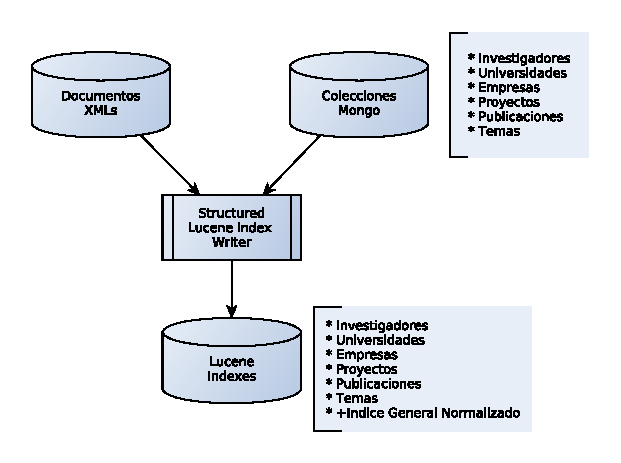
\includegraphics{graficos/LuceneIndexWriterEstructurado}
%   \caption{Lucene Index Writer para datos del proyecto Mitic}
%   \label{fig:LuceneIndexWriterEstructurado}
% \end{figure}

Para la construcción de indices lucene con los dumps de wikipedia usamos la librería gwtwiki (Ver Apéndice~\ref{sec:gwtwiki}).
Los artículos se indexan como documentos con los siguiente campos: \emph{id, title, body y all}. En este proceso se descartan artículos mal formados y 
entradas representado imágenes o discusiones, tal como se sugiere en la guía. 
Por mera curiosidad, tomamos tiempos en la contrucción de estos índices locales sobre versiones de wikipedia.
Estos son algunos tiempos de indexación para distintos dumps sobre una [[detalles de la compu]]:
\begin{center}
\begin{tabular}{| l | l | l | l |}
\hline
Idioma & Tamaño & \# Entradas & Tiempo \\ \hline
es & 50M & \# 16 millones & 2.5min \\ \hline
es & 50M & \# 16 millones & 2.5min \\ \hline
es & 50M & \# 16 millones & 2.5min \\ \hline
es & 50M & \# 16 millones & 2.5min \\ \hline
\end{tabular}
\end{center}

El proceso de creación de índices está ilustrado en la figura \ref{fig:LuceneIndexWriterBoth}



% \begin{figure}[H]
%   \centering
%     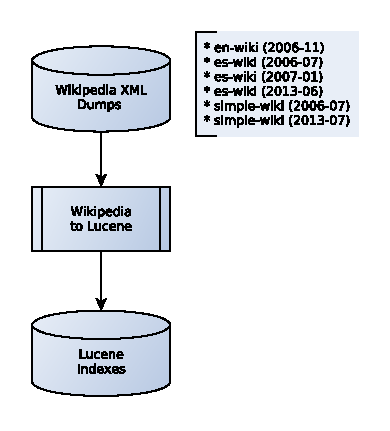
\includegraphics{graficos/LuceneIndexWriterWiki}
%   \caption{Lucene Index Writer para dumps de Wikipedia}
%   \label{fig:LuceneIndexWriterWiki}
% \end{figure}



\subsection{Interfaz de servicios}

La creación offline de índices lucene tiene como finalidad optimizar
la base de conocimiento para responder con mayor eficiencia 
a búsquedas de resultados en un momento posterior. 

En esta sección vamos a ver la interfaz que presenta la base de conocimientos indexada 
al resto de los módulos del sistema y qué dependencias existen con los módulos de
análisis lingüístico.

Para la base de conocimiento estructurada, reutilizamos un modelo de datos
escrito en java  del grafo de entidades que obtuvimos de los investigadores del proyecto mitic (Ver \ref{sec:modelos-morphia}).
A estos modelos se les agregó soporte para su representación como documento dentro de un índice.
Por ejemplo, el modelo para la entidad ``Universidad de Buenos Aires", además de
persistirse en la colección de universidades de la base de datos de mongo, también dispone de una representación como documento en 
un índice lucene particular (el índice de universidades) y otra en el índice general.
A nivel colecciones, cada entidad dispone de un representante que maneja el acceso a su colección en la base de datos y también a su índice. A partir de estos representantes por entidad que ofrecen acceso a una base de datos y a un índice creamos la interfaz \emph{KnowlegdeBase}. 
Cada entidad tiene una interfaz de administración de sus dos motores de persistencia. Las responsabilidades de esta interfaz son las de un handler de conocimiento acerca de una cierta clase de entidades. 
Además, esta interfaz permite la reificación de entidades implicitas en el modelo. Estas entidades son: Ciudad, Provincia, Centro de Investigación, etc \footnote{hacer y escribir bien}. Esta reificación significa abstraer las funciones directas contra la base de datos. Mientras el $KnowledgeBase$ de Investigadores habla directo contra la base mongo o contra lucene, el $KnowlegdeBase$ de Ciudades habla contra Investigadores, Universidades y Empresas verificando ciertos campos y recomponiendo la forma de la entidad, de modo abstracto y sin persistencia propia. 

[[Tablita con totales por entidad]]

\bigskip

[[Relaciones solo presentes en mongo]]

\bigskip

Las $KnowledgeBase$ de las cinco entidad y el índice general están, a su vez, controlados un $KnowlegdeManager$, que es la interfaz del módulo que maneja la base de conocimiento. 

El $KnowledgeManager$ ofrece diferentes servicios de verificación de entidades. Para una cadena de tokens cualquiera, este módulo puede decidir, con un cierto grado de confianza, los siguientes problemas:

\begin{itemize}
  \item Si la cadena de tokens es una entidad dentro del modelo de datos. Esto incluye:
    \begin{itemize}
      \item Es una entidad del modelo de datos: una universidad, una empresa, un investigador, un proyecto, una publicacion o una tematica
      \item Es una entidad inferida: una ciudad, una provincia, un centro de investigación, un lugar de trabajo
    \end{itemize}
  \item Si la cadena es una colección del modelo de datos, es decir, si se están nombrando \dblquote{Investigadores} o \dblquote{Universidades} como clase de entidades.
  \item Si la cadena es un atributo o una relación de una clase de entidades.
\end{itemize}

La primer verificación utiliza campos de identidad de las entidades y diferentes tipos de comparadores (Ver apéndice \allref{sec:comparadores} ). Cada entidad fue configurada con diferentes atributos de identidad y a su vez estos atributos están asociados a diferentes comparadores a con un cierto grado de peso y de confianza en el juicio general. 

La segunda y la tercera verificación utiliza estos mismos comparadores jerarquizados, pero compara las cadenas de entrada contra diccionario de sinónimos escrito a mano nombrando las diferentes clases de entidades y los atributos de cada una de ellas. 

\begin{figure}[H]
  \centering
    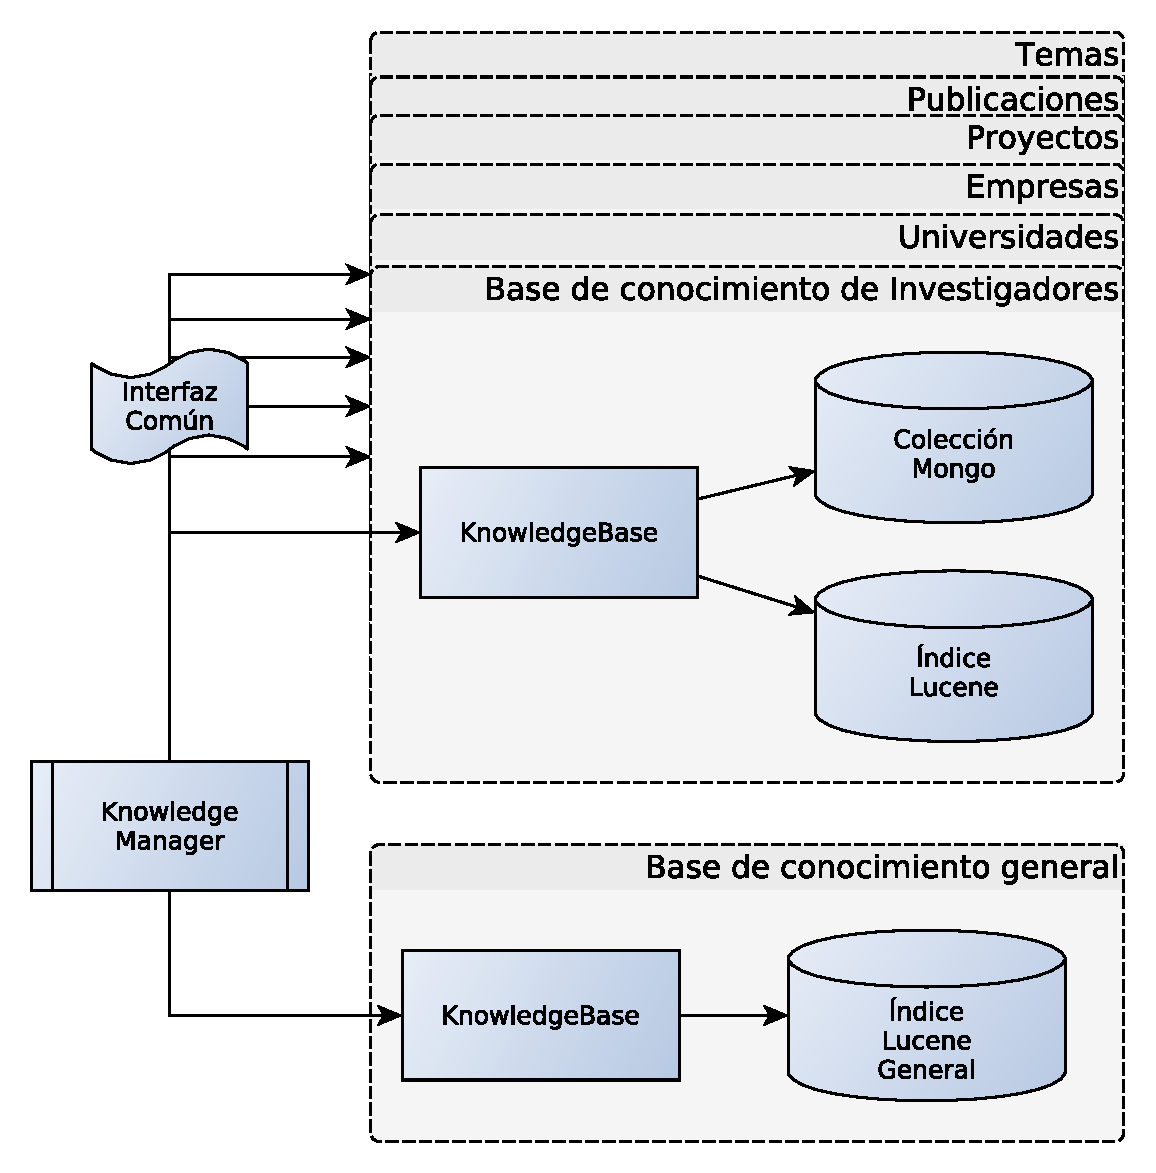
\includegraphics[scale=0.5]{graficos/KnowledgeManager}
  \caption{Base de Conocimiento de grafo de TICs}
  \label{fig:KnowledgeManager}
\end{figure}

\bigskip

La base de conocimiento de los ejercicios de Clef '07 es mucho más sencilla 
porque no existe ningún modelo \emph{a priori} más allá del documento de lucene.
El formato de la entidad ``artículo", como señalamos antes, es: $(id, titulo, cuerpo)$. 
En este caso, el trabajo más fino no está en el modelado inicial del dominio 
sino la capacidad lingüística de extraer pasajes a partir de un artículo y recomponer información
estructurada a partir de estos pasajes. Mientras que para un modelo estructurado la base de conocimiento
debería permitirnos, para un cierto input, identificar univocamente una entidad y darnos pistas sobre un pedido de
información acerca de esa entidad, el objetivo sobre un corpus de documentos en 
traer todos los documentos en los que sea posible que exista un pasaje respondiendo a la pregunta o
evidencia relevante para apoyar una respuesta. Es decir, mientras una respuesta acotada es una virtud para
el manejador de una base de conocimientos estructurada, el manejador de una lista de documentos de texto debería devolver
una lista lo suficientemente grande para contener la respuesta dentro de los pasajes. La razón de esta política es que si
por ser demasiado estrictos a la hora de retornar documentos llegasemos a descartar un pasaje candidato válido esto
redundaría en una baja generar de efectividad, mientras que en pasos subsiguiente será trivial descartar toda información irrelevante
sin tanto costo. Por eso, el acceso a los indices de wikpedia consta simplemente de un generador de queries similar al recién comentado
accediendo y acumulando resultados (rankeados) a partir de un $LuceneIndexReader$ común (Ver \ref{sec:lucene} \nameref{sec:lucene} para más información).


\bigskip

\section{Análisis de la pregunta}

En este paso se realizan diferentes análisis lingüísticos de la pregunta.
El resultado son distintas características asociadas a la pregunta (anotaciones)
y distintas entidades semánticas reconocidas útiles para el proceso de generación de respuestas. 
Las herramientas de procesamiento de lenguaje natural que utilizamos en 
la implementación de este paso del pipeline 
incluyen: detección de lenguaje, extracción y verificación de entidades nombradas (NER), 
de verbos, sustantivos, qwords (qué, quién, cómo) (POS), análisis de n-gramas y categorización por tipo de pregunta (QC).

El proceso de análisis de la pregunta es bastante similar para ambos approachs (estructurado y no estructurado), por lo
que comentaremos ambos en simultaneo, mencionando diferencias cuando corresponda. 
Estructuraremos esta parte de la tesis en las siguientes secciones:

\begin{itemize}
\item Detección de idioma 
\item Detección y verificación de entidades nombradas
\item Análisis gramatical
\item Clasificación del tipo de pregunta
\end{itemize}

Si bien es cierto que el segundo item está basado principalmente en NER-tagging, el tercero en POS-tagging y el cuarto en Question Clasiffication, 
cada uno de estos pasos utiliza estas herramientas de diferentes maneras. Por ejemplo, para la detección y verificación de entidades del analisis estructurado, además del NER-tagger también utilizamos la base de conocimiento y el análisis gramatical y, para el español, la clasificación del tipo de pregunta se hace apoyandose en las qwords identificadas por el POS-tagger.

\subsection{Idioma}

\begin{figure}
  \centering
    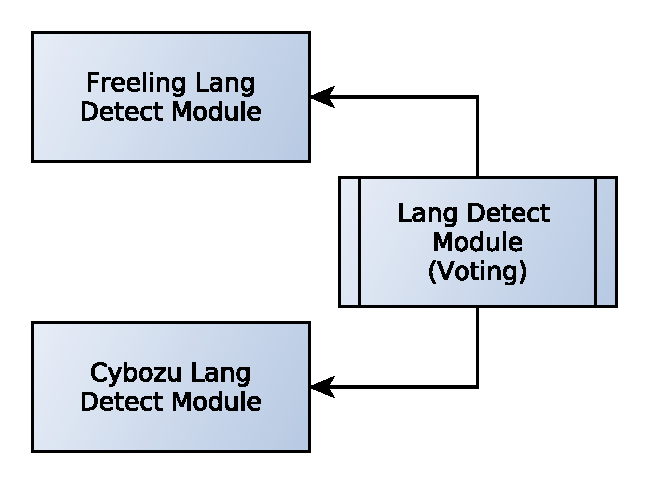
\includegraphics[scale=0.86]{graficos/LangDetect}
  \caption{Módulo de Detección de Idiomas}
  \label{fig:LangDetect}
\end{figure}

El módulo de detección de idiomas de nuestro sistema utiliza dos librerías distintas.
El módulo de detección de idiomas de Freeling y una librería especializada de Cybozu Labs. (Ver apéndices \allref{sec:freeling} y \allref{sec:cybozu} para más información)

Ambos permiten priorizar la detección de ciertos idiomas sobre otros desde su configuración.
De esta manera podemos forzarlos a identificar sólo los idiomas esperados en nuestro dominio. 
Ambos fueron configurados para detectar inglés y español para mejorar la confiabilidad,
pero pueden habilitarse más idiomas de ser necesario y funcionan correctamente. 

El módulo de detección simplemente evalua ambos algoritmos y 
decide el resultado con un cierto grado de confianza. En caso de existir un empate, se 
prioriza la opción de Cybozu labs que en la práctica dió resultados más exactos.

De todos modos, el problema "detección de idioma" no introduce mayores complicaciones y parece un problema bien resulto.
Es decir, la mayoría de las veces ambos módulos responden lo mismo y de modo correcto.
Sin embargo, para ciertos casos bordes molestos (pero lamentablemente frecuentes)
el detector de Cybozu resultó funcionar mejor. Por ejemplo, está el caso de la pregunta formulada en inglés pero acerca de una entidad nombrada en español: 
``Where is located the Universidad de Buenos Aires?". Este problema está particularmente presente en el procesamiento de preguntas -nuestra tarea-, dado que son textos cortos en los que una construcción sustantivada en otro idioma puede desequilibrar erróneamente la balanza. 

A continuación presentamos algunos ejemplos que ilustran el funcionamiento de ambas librerías y el resultado final de nuestro módulo en estos casos:

\begin{center}
\begin{tabular}{| p {8cm} | l | l | l |}
\hline
Texto & Freeling & Cybozu & Resultado \\ \hline
¿Dónde queda la Universidad de Buenos Aires? & es & es & es \\ \hline
Where is located the University of Buenos Aires? & en & en & en \\ \hline
Where is located the Univesidad de Buenos Aires? & en & en & en \\ \hline
Where is located Universidad de Buenos Aires? &  {\color{red}es} & en & en \\ \hline
Quién es Carolina Fernandez? & es & es & es \\ \hline
Who is Carolina Fernandez? &  {\color{red}none} & en & en \\ \hline
Quién es John McCain? & {\color{red}none} & es & es \\ \hline
Who is John McCain? & en & en & en \\ \hline
Dónde vive John McCain y por qué vive allí? & es & es & es \\ \hline
Where does Carolina Fernandez live and why does she lives there? & en & en & en \\ \hline
\end{tabular}
\end{center}

Los ejercicios de Clef '07 no evaluan detección de idiomas. Los archivos de preguntas están separadas por idioma y no se espera que el idioma se infiera a partir de los textos de las preguntas, sino que es un dato dado al sistema de QA.

\subsection{Entidades nombradas}
\label{subsec:impl-ner}

Para la detección de entidades utilizamos la clase simple de detección (NER) y clasificación (NEC) de entidades de Freeling y el NERC de Stanford (ver \allref{sec:freeling} y \allref{sec:stanford-ner}). Las herramientas de Stanford en general superan a las de Freeling -al igual que el detector de idiomas de Cybozu-, pero solo sirven para inglés. La clasificación utilizada por ambos es la más general de las comentadas en \allref{subsec:nerc}: persona, lugar, organización y otros. 

Veamos algunos ejemplos de funcionamiento de los módulos de detección de idiomas. 

\begin{center}
\begin{tabular}{| p {8cm} | l | l | l |}
\hline
Texto & Freeling & Cybozu & Resultado \\ \hline
¿Dónde queda la Universidad de Buenos Aires? & es & es & es \\ \hline
Where is located the University of Buenos Aires? & en & en & en \\ \hline
Where is located the Univesidad de Buenos Aires? & en & en & en \\ \hline
Where is located Universidad de Buenos Aires? &  {\color{red}es} & en & en \\ \hline
Quién es Carolina Fernandez? & es & es & es \\ \hline
Who is Carolina Fernandez? &  {\color{red}none} & en & en \\ \hline
Quién es John McCain? & {\color{red}none} & es & es \\ \hline
Who is John McCain? & en & en & en \\ \hline
Dónde vive John McCain y por qué vive allí? & es & es & es \\ \hline
Where does Carolina Fernandez live and why does she lives there? & en & en & en \\ \hline
\end{tabular}
\end{center}

\medskip

Mientras la detección de entidades para los ejercicios de Clef se detiene en el reconocimiento de entidades nombradas a nivel lingüísitico, para el sistema estructurado el proceso es un poco más complejo. Esto se debe a que en este caso la detección de entidades es esencial. Si en el proceso de anotado de la pregunta no se logra identificar alguna entidad reconocida por el modelo de datos, entonces se está muy lejos de encontrar una respuesta. Por eso, además de utilizar los modulos NER recién mencionado, agregamos otros algoritmos de detección y, también, verificación de entidades. 

En principio, verificamos la o las entidades nombradas reconocidas contra la base de conocimiento. El $KnowledgeManager$ ofrece diferentes servicios de verificación de entidades. Para una cadena de tokens cualquiera, este módulo puede decidir, con un cierto grado de confianza, si:

\begin{itemize}
  \item La cadena de tokens es una entidad dentro del modelo de datos. Esto incluye:
    \begin{itemize}
      \item Es una entidad del modelo de datos: una universidad, una empresa, un investigador, un proyecto, una publicacion o una tematica
      \item Es una entidad inferida: una ciudad, una provincia, un centro de investigación, un lugar de trabajo
    \end{itemize}
  \item La cadena es una colección del modelo de datos, es decir, si se están nombrando \dblquote{Investigadores} o \dblquote{Universidades} como clase de entidades.
  \item La cadena es un atributo o una relación de una clase. (nombre de investigador)
\end{itemize}

Parte importante del trabajo para este esquema es lograr identificar este tipo de entidades lingüísticas, por lo que además de verificar los resultados del proceso de NER-tagging, también generamos otras cadenas de input. Notar además que los nombres de clase y de atributos de clase no tendrían por que ser reconocidas por el NER-tagger. Por ejemplo, para ``¿Qué investigadores trabajan en Córdoba?", \dblquote{investigadores} está haciendo referencia al nombre de una clase pero no es el tipo de entidades lingüísticas que detecta un NER-tagger. 

Por estas razones, generamos más entidades lingüísticas posibles además de las entidades detectadas por los NER-taggers. Una vez que todas las entidades nombradas fueron verificadas, generamos n-gramas sobre el resto de la pregunta para chequear por más tokens reconocibles. Configuramos la generación de n-gramas de 1 a 3, con ciertos filtros para no verificar construcciones que no representan entidades de manera trivial. Por ejemplo: dejamos sólo los unigramas que cumplan el rol de sustantivos, eliminamos bigramas que sean un sustantivo y una acción, salteamos NERs ya reconocidas, etre otros.


\subsection{Análisis gramatical}

De las diferentes etiquetas que generan los POS-taggers, en nuestro sistema distinguimos los verbos, los sustantivos, las qwords y las palabras triviales. 
Las palabras etiquetadas cumplen distintos roles a lo largo del proceso de generación de respuestas. Como señalamos recién, los n-gramas que se verifican contra la base de datos están filtrados por los roles gramaticales de sus tokens. Por otro lado, a la hora de generar el tipo de pregunta para una pregunta en español, utilizamos, como mecanismo ad-hoc, las qwords. 

\begin{center}
\begin{tabular}{| l | l |}
\hline
Clase & Ejemplos\\ \hline
qword  & qué, quién, cómo, dónde, cuándo\\ \hline
verbo & trabaja, trabajar, trabajando \\ \hline
trivial  & lo, a, de, y \\ \hline
sustantivos  & universidad, impresora, álgebra \\ \hline
\end{tabular}
\end{center}

Los usos más intensivos de estas etiquetas son el filtrado de n-gramas que describimos en la sección anterior para el caso estructurado (\allref{subsec:impl-ner}), un algoritmo ad-hoc de etiquetado de Q-Type para el caso español (es el próximo tema a discutir en \allref{subsec:qtype}) y, para la generación de respuestas, las ponderaciones de pasajes en los scorers de los ejercicios de Clef (\allref{subsec:scorers}), y finalmente, sirven para desempatar por atributos o relaciones preguntadas en algunos casos del modelo estructurado.

\subsection{Clasificación}
\label{subsec:qtype}


\section{Generación de Respuestas}

\subsection{Estructurado}
Si en el paso 8 se procesaron menos del 80\% de los tokens de la
palabra, el sistema se da 

por vencido y devuelve una lista de score docs.

Si no, realiza un análisis estructurado basándose en la
información obtenida.


Una vez completada la generación de
metadatos lingüísticos, se procede al tercer paso, que toma
diferentes formas dependiendo de la información encontrada en el
análisis de la pregunta.


Dependiendo de cuánto se haya procesado de la pregunta original,
existen dos tipos de flujos distintos de generación de respuestas: el
estructurado y el no estructurado.

La generación de respuestas estructurada se construye cuando la
información obtenida en el análisis lingüístico es suficiente
para generar un mapeo coherente a la ontología definida
implícitamente por la base de conocimientos. El análisis no
estructurado se ejecuta cuando la información generada no fue
suficiente y consiste en intentar ubicar marcas que puedan reconducir
al análisis al flujo estructurado (es decir, se intentan diferentes
transformaciones a fin de identificar información que permita el
análisis estructurado). Esto se realiza con métodos menos
confiables y menos rápidos que en el análisis lingüístico
inicial. Si el análisis falla en esta segunda barrera, se procede a
dar una respuesta ad-hoc con la información disponible. 

En flujo de respuesta estructurado depende de la cantidad de
información que se haya identificado. Esta información, en este
punto, tiene tres tipos: QType, NERs y verbos. 

\subsection{No Estructurado}

\subsubsection{Scorers}
\label{subsec:scorers}


\begin{figure}
  \centering
    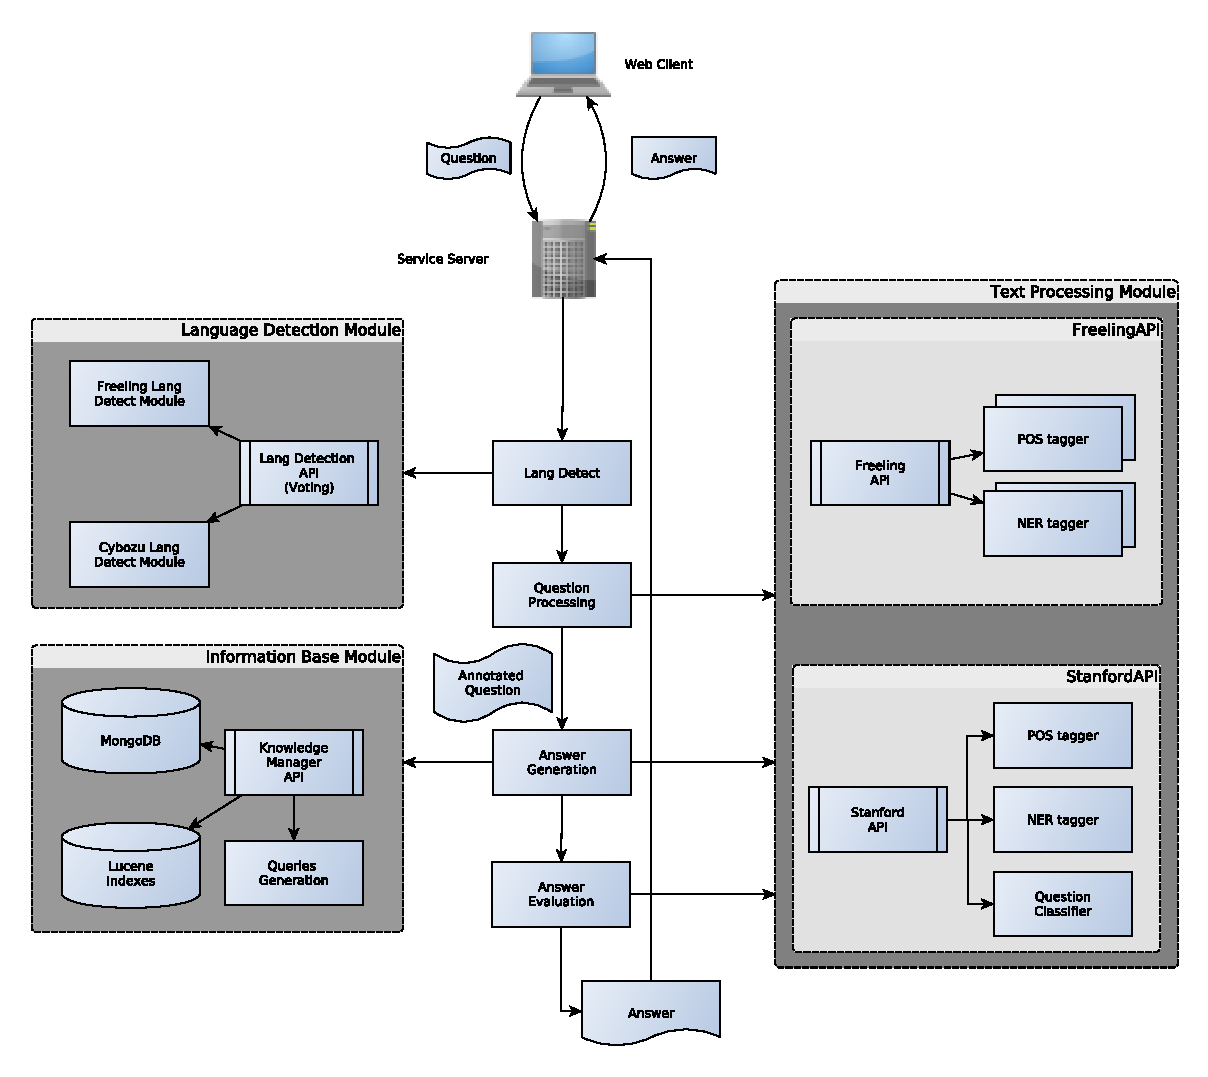
\includegraphics[scale=0.86]{graficos/Architecture}
  \caption{Arquitectura}
  \label{fig:Architecture}
\end{figure}

Como dice en \cite{greenwade93} y también en \cite{RE1}
%\end{document}
